\documentclass[a4paper,twoside]{article}
\usepackage[T1]{fontenc}
\usepackage[bahasa]{babel}
\usepackage{graphicx}
\usepackage{graphics}
\usepackage{amsfonts}
\usepackage{float}
\usepackage[cm]{fullpage}
\pagestyle{myheadings}
\usepackage{etoolbox}
\usepackage{setspace} 
\usepackage{lipsum} 
\usepackage{subcaption}
\usepackage{amsmath}
\usepackage{enumitem}
\setlength{\headsep}{30pt}
\usepackage[inner=2cm,outer=2.5cm,top=2.5cm,bottom=2cm]{geometry} %margin
% \pagestyle{empty}

\makeatletter
\renewcommand{\@maketitle} {\begin{center} {\LARGE \textbf{ \textsc{\@title}} \par} \bigskip {\large \textbf{\textsc{\@author}} }\end{center} }
\renewcommand{\thispagestyle}[1]{}
\markright{\textbf{\textsc{Laporan Perkembangan Pengerjaan Skripsi\textemdash Sem. Ganjil 2020/2021}}}

\onehalfspacing
 
\begin{document}

\title{\@judultopik}
\author{\nama \textendash \@npm} 

%ISILAH DATA BERIKUT INI:
\newcommand{\nama}{Cristopher}
\newcommand{\@npm}{2017730017}
\newcommand{\tanggal}{12/01/2021} %Tanggal pembuatan dokumen
\newcommand{\@judultopik}{Identifikasi Pergerakan Kolektif Pada Data Pejalan Kaki} % Judul/topik anda
\newcommand{\kodetopik}{LNV4902}
\newcommand{\jumpemb}{1} % Jumlah pembimbing, 1 atau 2
\newcommand{\pembA}{Lionov Wiratma}
\newcommand{\pembB}{-}
\newcommand{\semesterPertama}{49 - Ganjil 20/21} % semester pertama kali topik diambil, angka 1 dimulai dari sem Ganjil 96/97
\newcommand{\lamaSkripsi}{1} % Jumlah semester untuk mengerjakan skripsi s.d. dokumen ini dibuat
\newcommand{\kulPertama}{Skripsi 1} % Kuliah dimana topik ini diambil pertama kali
\newcommand{\tipePR}{B} % tipe progress report :
% A : dokumen pendukung untuk pengambilan ke-2 di Skripsi 1
% B : dokumen untuk reviewer pada presentasi dan review Skripsi 1
% C : dokumen pendukung untuk pengambilan ke-2 di Skripsi 2

% Dokumen hasil template ini harus dicetak bolak-balik !!!!

\maketitle

\pagenumbering{arabic}

\section{Data Skripsi} %TIDAK PERLU MENGUBAH BAGIAN INI !!!
Pembimbing utama/tunggal: {\bf \pembA}\\
Pembimbing pendamping: {\bf \pembB}\\
Kode Topik : {\bf \kodetopik}\\
Topik ini sudah dikerjakan selama : {\bf \lamaSkripsi} semester\\
Pengambilan pertama kali topik ini pada : Semester {\bf \semesterPertama} \\
Pengambilan pertama kali topik ini di kuliah : {\bf \kulPertama} \\
Tipe Laporan : {\bf \tipePR} -
\ifdefstring{\tipePR}{A}{
			Dokumen pendukung untuk {\BF pengambilan ke-2 di Skripsi 1} }
		{
		\ifdefstring{\tipePR}{B} {
				Dokumen untuk reviewer pada presentasi dan {\bf review Skripsi 1}}
			{	Dokumen pendukung untuk {\bf pengambilan ke-2 di Skripsi 2}}
		}
		
\section{Latar Belakang}

Bergerak merupakan sebuah aktivitas yang selalu kita temui setiap saat. Segala sesuatu yang ada di sekitar kita selalu bergerak untuk mencapai tujuan tertentu. Manusia selalu bergerak untuk melakukan aktivitas sehari-hari. Berbagai jenis hewan melakukan migrasi untuk mencari lingkungan baru yang lebih mampu untuk menunjang kehidupan. Tanaman dapat bergerak melalui fototropisme yang menyebabkan tanaman bertumbuh mengikuti arah sinar matahari. Bahkan, bumi selalu berputar mengelilingi porosnya yang menyebabkan pergantian hari. Dapat dikatakan bahwa bergerak merupakan aktivitas yang tak dapat dilepaskan dari kehidupan sehari-hari. Hal tersebut menumbuhkan rasa ketertarikan manusia untuk mengumpulkan, menyelidiki, serta mempelajari segala aspek mengenai pergerakan. Sayangnya, sedikitnya sumber dan cara mendapatkan data menghambat penelitian mengenai pergerakan di masa lalu.

\iffalse

\begin{figure}[h]
    \centering
    \begin{subfigure}[b]{0.45\textwidth}
        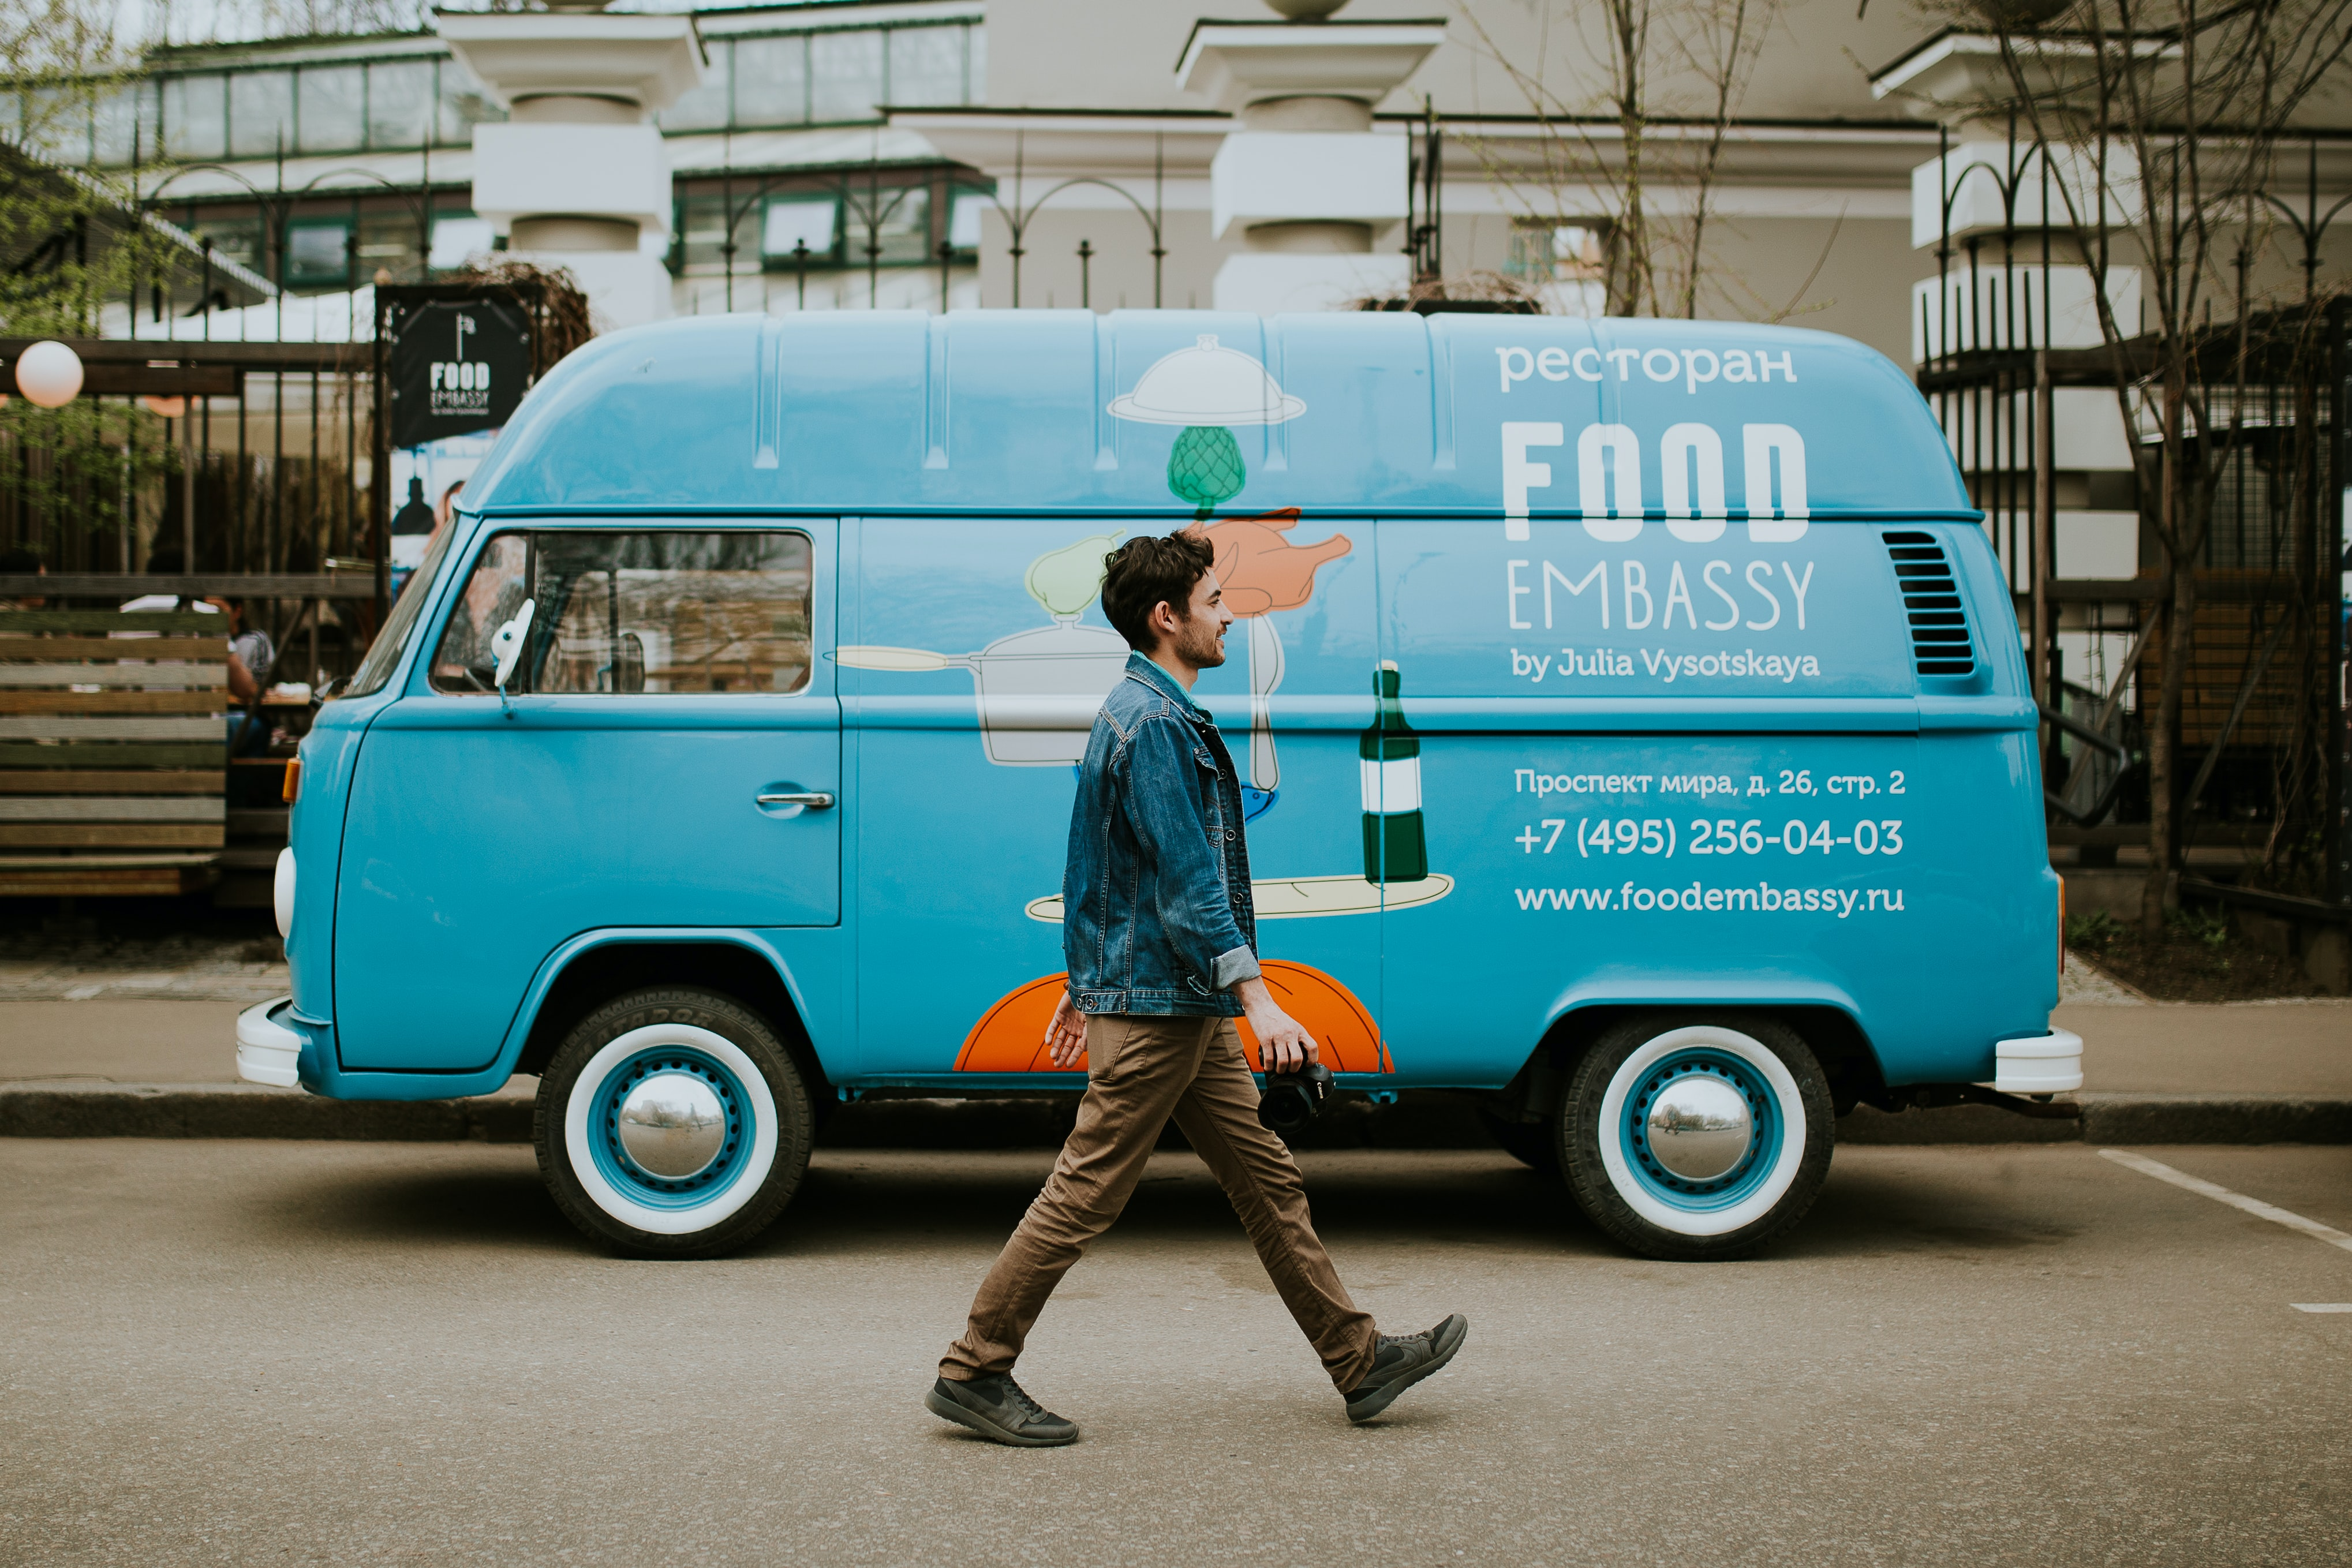
\includegraphics[width=\textwidth, height=5cm]{Gambar/bergerak.jpg}
        \caption{Manusia bergerak untuk memenuhi kebutuhan sehari-hari\protect\footnotemark}
        \label{bab1:manusia}
    \end{subfigure}
    \begin{subfigure}[b]{0.45\textwidth}
        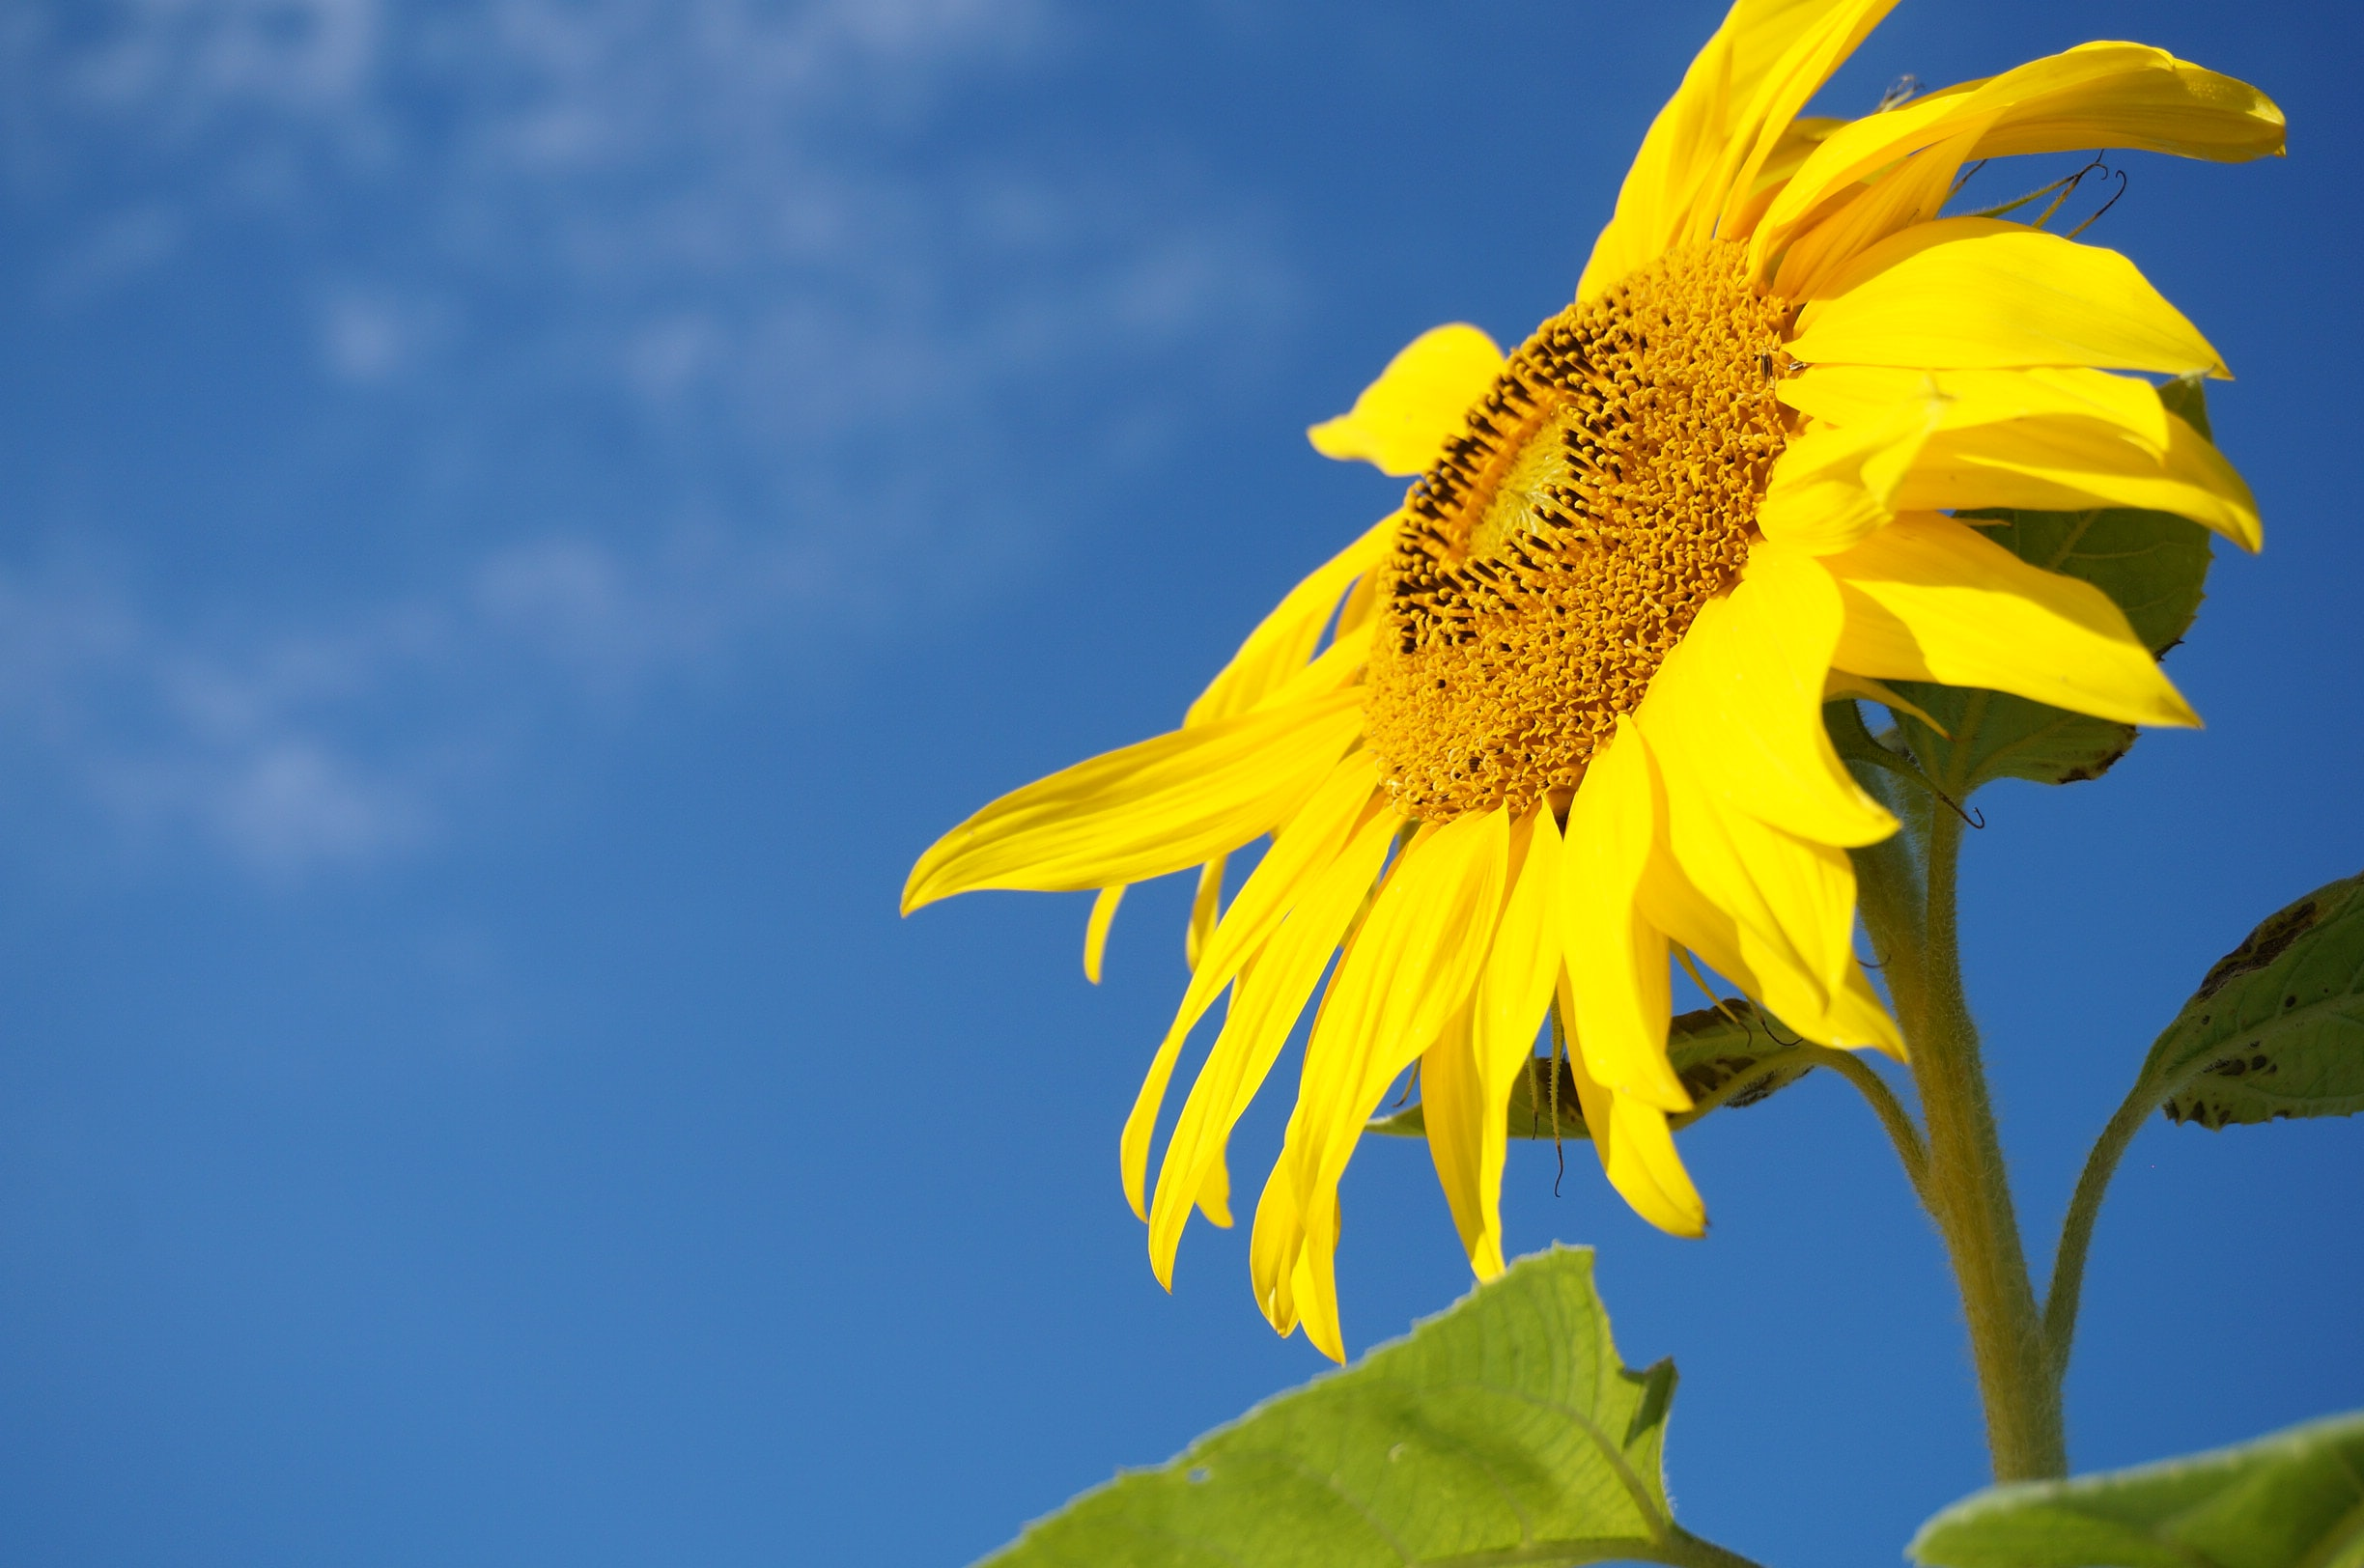
\includegraphics[width=\textwidth, height=5cm]{Gambar/sunflower.jpg}
        \caption{Bunga matahari bertumbuh mengikuti arah sinar matahari\protect\footnotemark}
        \label{bab1:sunflower}
    \end{subfigure}
    \caption[Aktivitas pergerakan]{
    Aktivitas pergerakan yang dilakukan oleh berbagai entitas di sekitar kita}
    \label{bab1:pergerakan}
\end{figure}

\footnotetext{Alvin Mamudov,  2017, diakses pada tanggal 4 Januari 2021, \url{https://unsplash.com/photos/FlLHbmF3AHc}.}

\footnotetext{Lisa Pellegrini, 2016, diakses pada tanggal 4 Januari 2021, \url{https://unsplash.com/photos/XCvy_eufErI}.}

\fi

Seiring berjalannya waktu, kemunculan teknologi modern seperti \textit{Geographic Information System} (GIS) menyebabkan data pergerakan yang bersumber dari berbagai entitas menjadi semakin banyak dan semakin mudah didapatkan. Hal tersebut memicu kembalinya pertumbuhan minat penelitian mengenai pergerakan oleh berbagai peneliti dalam berbagai bidang. Terdapat banyak hal menarik yang dapat dimanfaatkan melalui analisis terhadap data pergerakan. Salah satu contoh nyata dari pemanfaatan analisis data pergerakan adalah analisis pergerakan bebek domestik, di mana melalui data pergerakan bebek, virolog dapat mengidentifikasi daerah-daerah yang memiliki risiko persebaran flu burung yang tinggi.

Dalam sebuah pergerakan, setiap entitas yang bergerak memiliki lintasan. Lintasan merupakan jalur yang dilalui oleh entitas selama melakukan pergerakan dalam rentang waktu tertentu. Data mengenai lintasan yang ditempuh oleh entitas yang bergerak bersifat kontinu. Data lintasan dapat diperoleh melalui berbagai cara, di mana hal tersebut ditentukan oleh tipe entitas, lingkungan tempat terjadinya pergerakan, teknologi yang digunakan, dan lain sebagainya. Sekarang ini, data mengenai lintasan biasanya diperoleh melalui sistem modern seperti sistem Argos-Doppler dan \textit{global positioning system} (GPS) yang lazim ditemukan pada telepon pintar, di mana keduanya sama-sama memanfaatkan teknologi satelit. Kedua sistem tersebut memiliki beberapa kelebihan dibandingkan penggunaan cara-cara tradisional seperti memiliki akurasi yang jauh lebih baik, mampu memperoleh lebih banyak data lintasan dari berbagai entitas sekaligus, dapat dikustomisasi sesuai kebutuhan, dan masih banyak lagi.

Sayangnya, perkembangan teknologi tetap tidak mampu untuk merekam data lintasan secara sempurna. Hal tersebut menyebabkan data lintasan yang diperoleh tidak bersifat kontinu seperti yang diharapkan, melainkan bersifat diskrit. Berdasarkan sifat tersebut, data lintasan yang diperoleh akan direpresentasikan sebagai catatan posisi dari entitas yang bergerak yang diurutkan berdasarkan titik waktu. Secara formal, lintasan merupakan kumpulan dari pasangan posisi-waktu $(p_0, t_0), (p_1, t_1), \ldots, (p_x, t_x)$, di mana $p_i$ merupakan posisi entitas yang relatif terhadap ruang gerak entitas pada titik waktu $t_i$. Pada umumnya, entitas akan bergerak dalam sebuah ruang \textit{euclidean} dua dimensi atau tiga dimensi yang masing-masing dapat direpresentasikan sebagai 
$\mathbb{R}^2$ dan $\mathbb{R}^3$.

Setiap lintasan memiliki atribut-atribut dengan nilai tertentu sebagai karakteristik yang membedakan satu lintasan dengan lintasan lain. Atribut-atribut tersebut kemudian dapat diolah menjadi ukuran lintasan yang memiliki kegunaan yang lebih spesifik. Analisis terhadap data pergerakan selalu memanfaatkan setidaknya salah satu ukuran yang terdapat pada data lintasan. Sebagai contoh, kecepatan dapat digunakan untuk mengukur pengaruh angin pada pergerakan burung.

Terdapat berbagai jenis analisis yang dapat dilakukan pada data pergerakan seperti segmentasi lintasan, pengukuran kemiripan lintasan, \textit{clustering} pada entitas yang bergerak, dan identifikasi pola pergerakan kolektif yang menjadi fokus utama pada skripsi ini. Tujuan dari analisis pola pergerakan kolektif adalah mengidentifikasi kelompok pergerakan yang terbentuk dari entitas-entitas yang bergerak bersama dalam rentang waktu yang cukup lama. Analisis pola pergerakan kolektif memiliki pemanfaatan dalam berbagai bidang. Sebagai contoh, identifikasi pola pergerakan kolektif dapat dimanfaatkan pada bidang keamanan untuk mengidentifikasi pergerakan mencurigakan dari sekelompok orang.

\iffalse

\begin{figure}[h]
    \centering
    \begin{subfigure}[h]{0.45\textwidth}
        \centering
        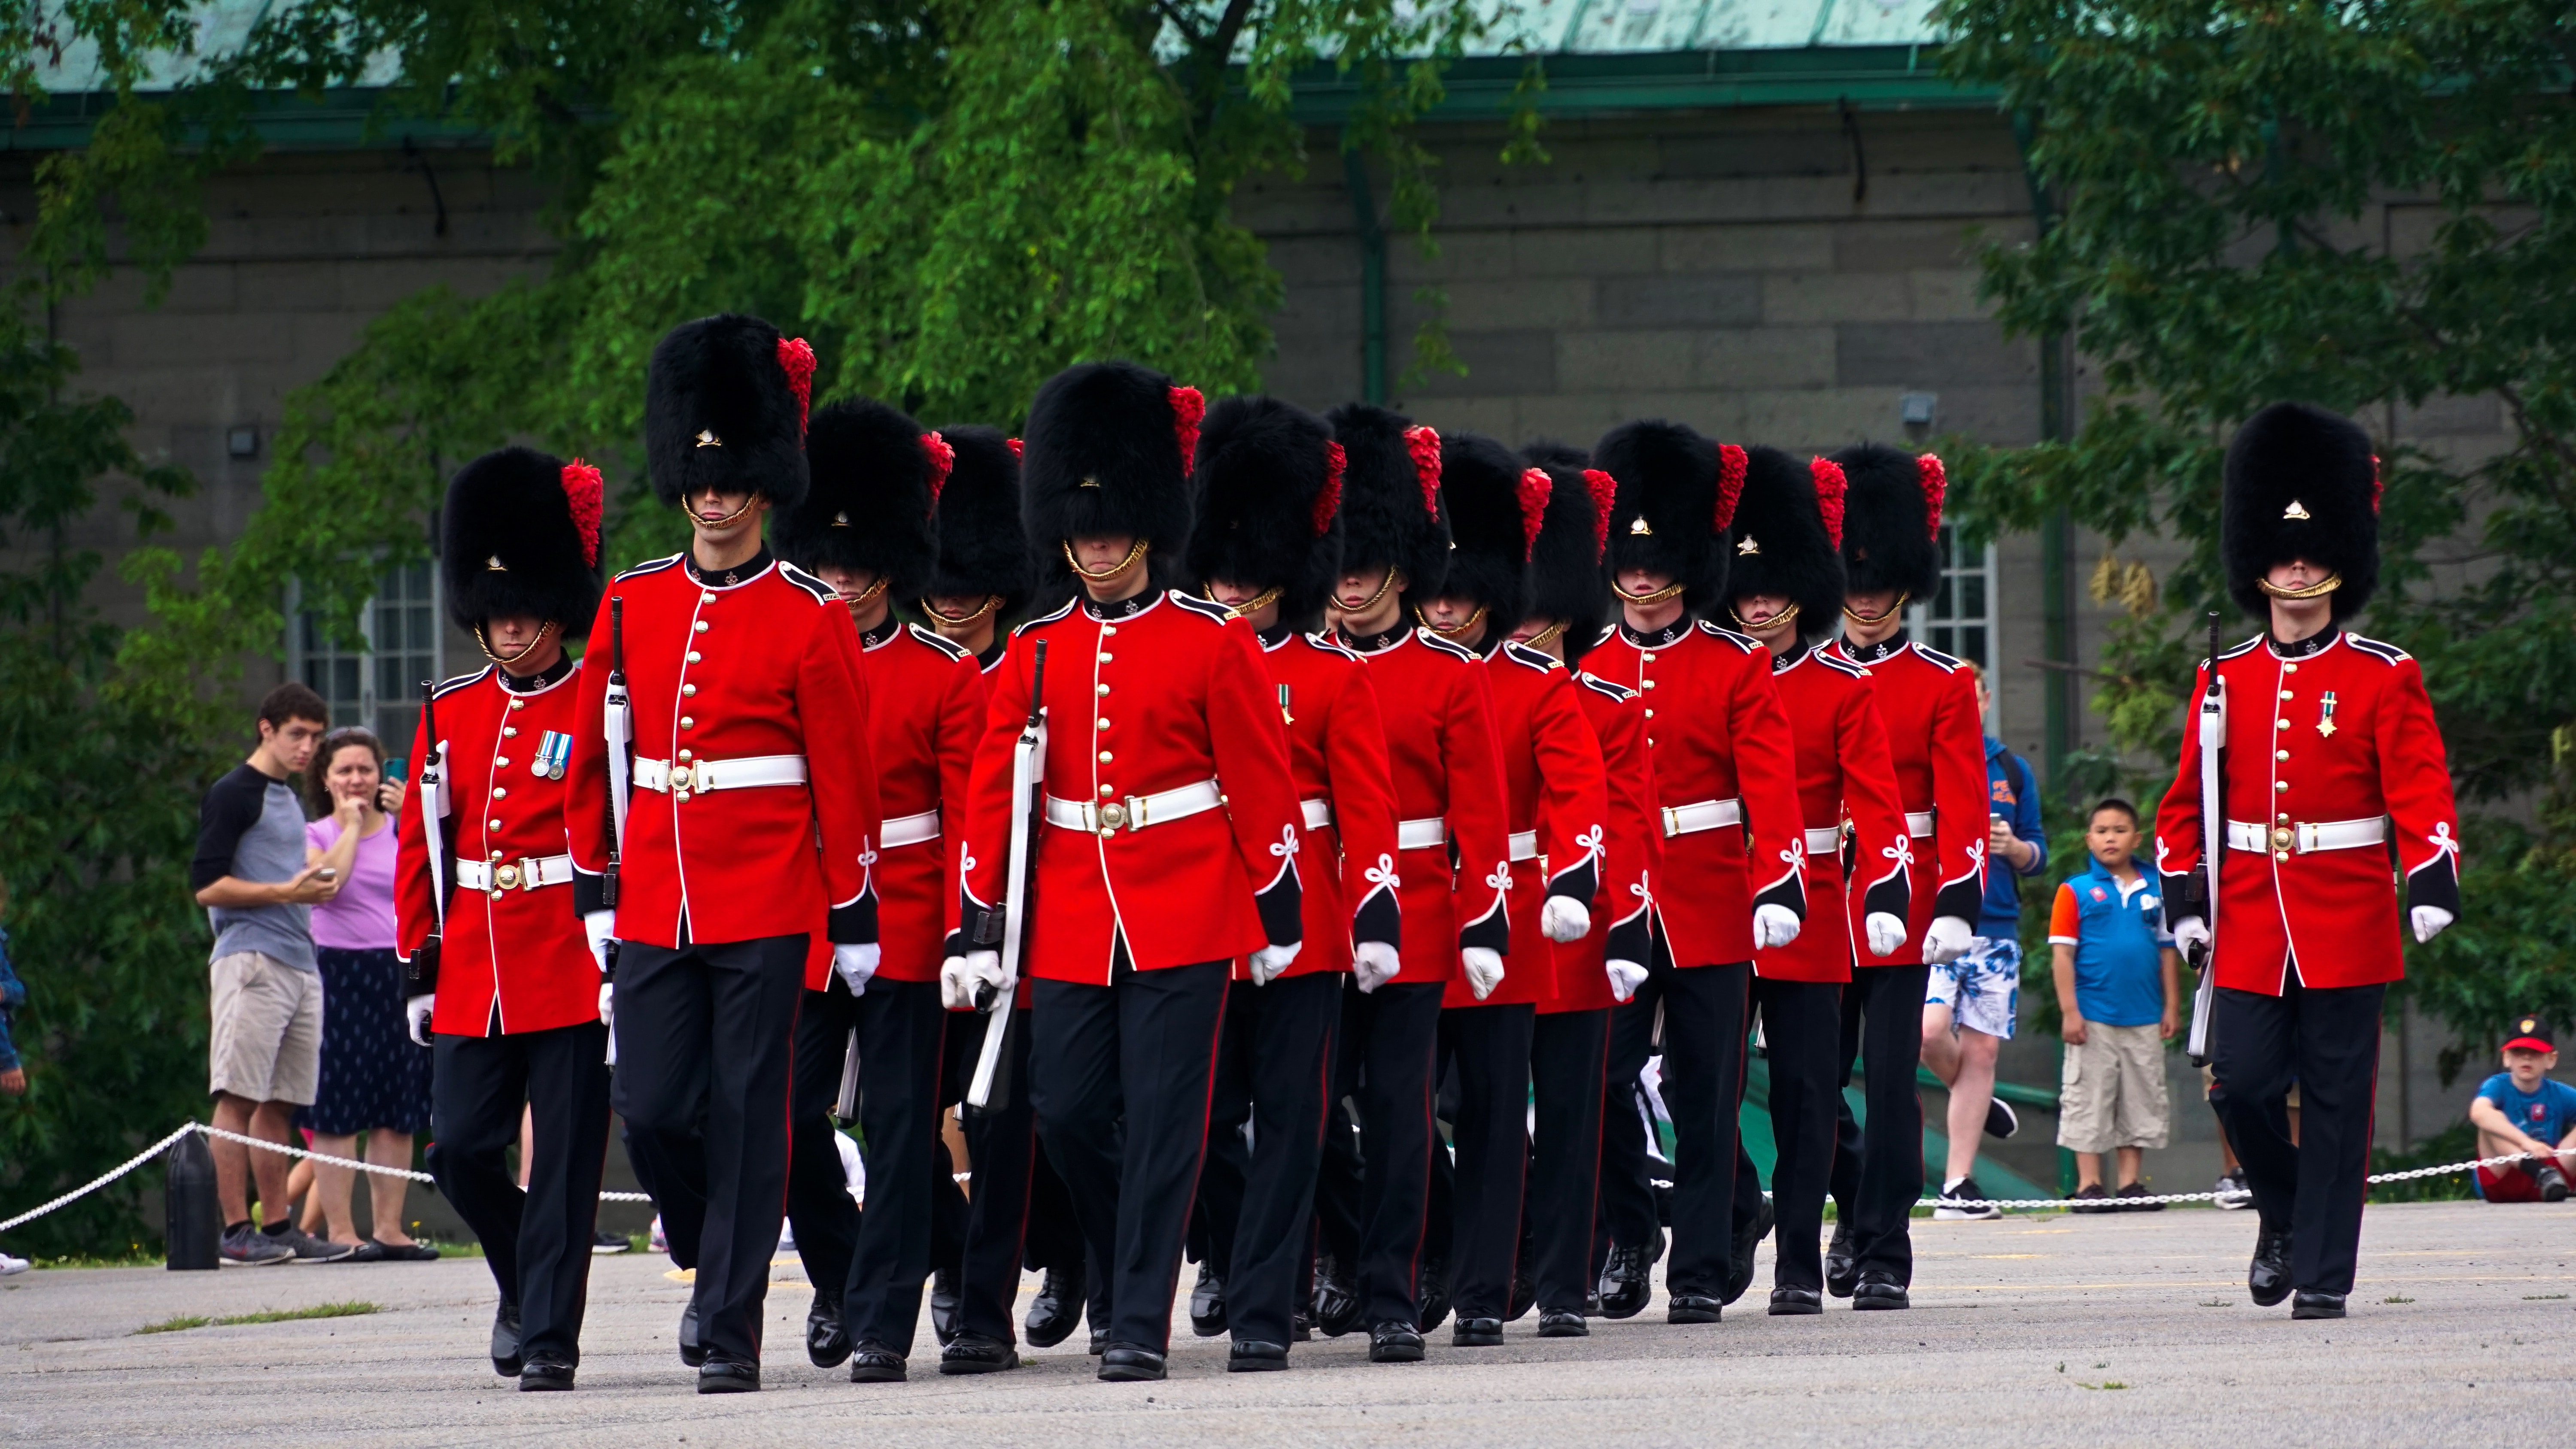
\includegraphics[width=\textwidth, height=4.5cm]{Gambar/army.jpg}
        \caption{Kumpulan tentara bergerak bersama membentuk sebuah regu\protect\footnotemark}
    \end{subfigure}
    \begin{subfigure}[h]{0.45\textwidth}
        \centering
        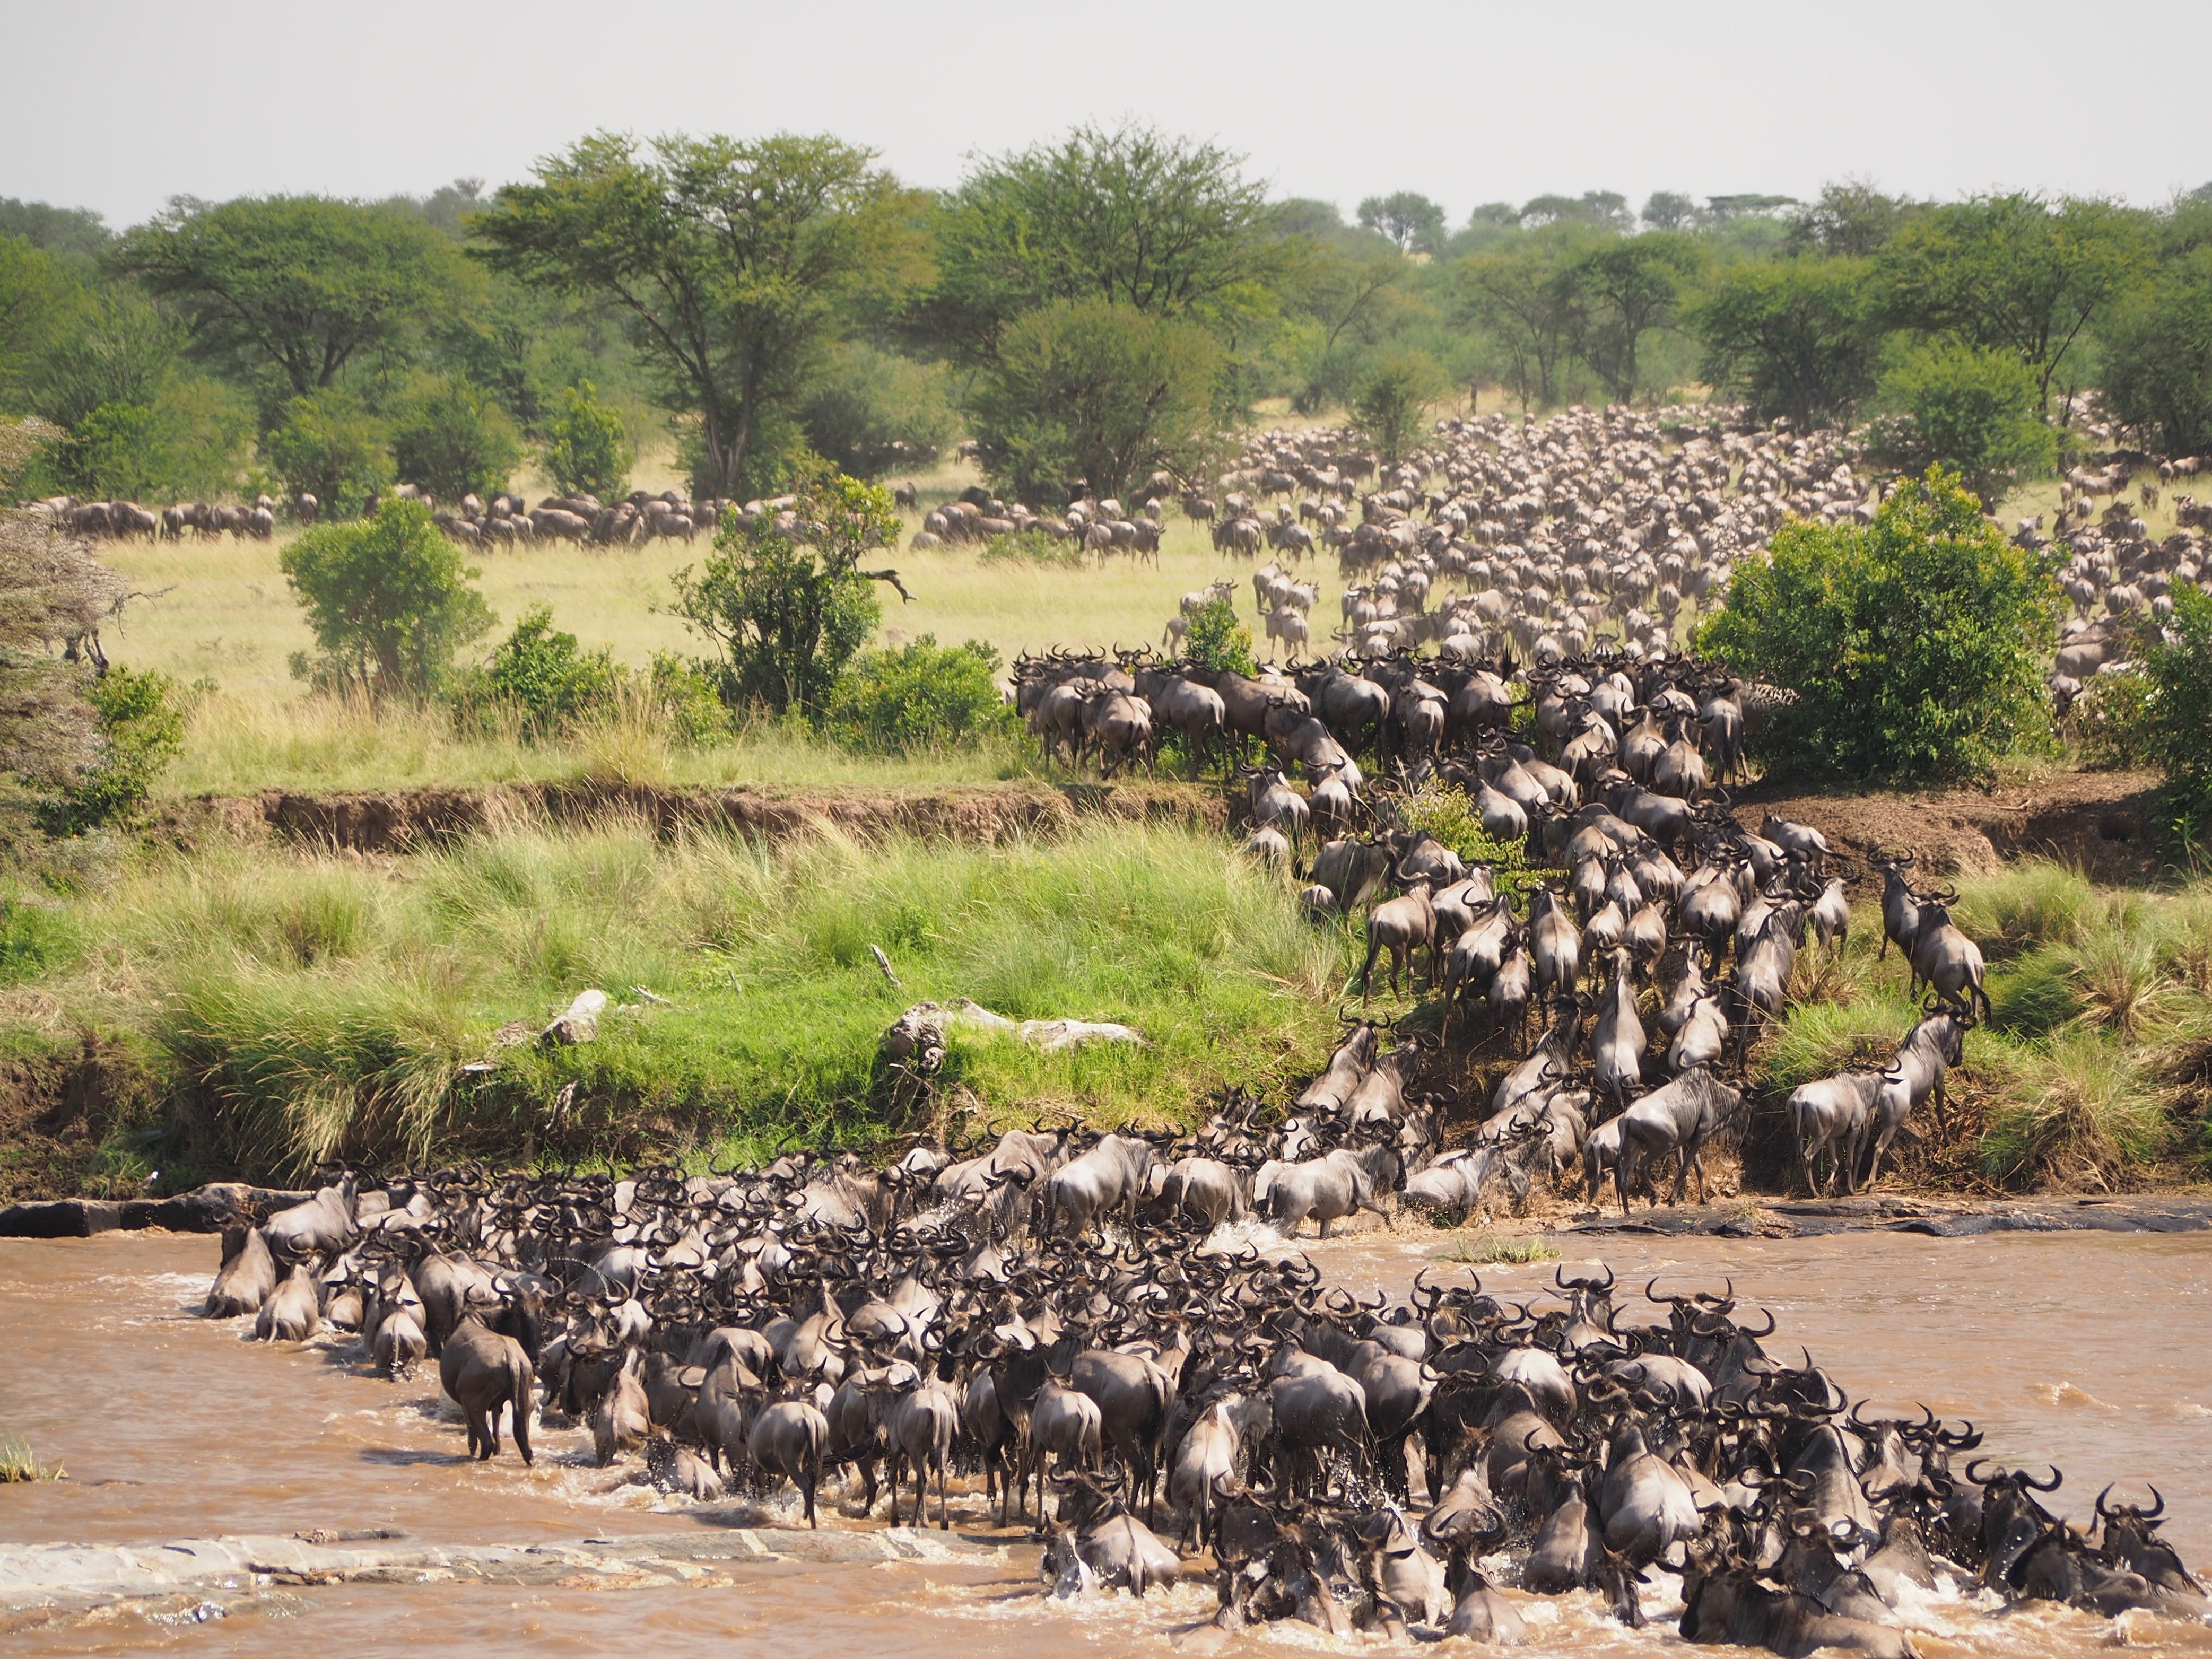
\includegraphics[width=\textwidth, height=4.5cm]{Gambar/wildebeest.jpg}
        \caption{Kawanan \textit{wildebeest} membentuk \textit{herd} untuk melakukan migrasi musiman\protect\footnotemark}
    \end{subfigure}
    \caption[Pergerakan kolektif dunia nyata]{Pergerakan kolektif yang sering kita temui di dunia nyata}
    \label{bab1:collective-movement}
\end{figure}

\footnotetext{Damon On Road, \textit{C\'{e}r\'{e}monie militaire du Man\`{e}ge militaire du Qu\'{e}bec}, 2020, diakses pada tanggal 4 Januari 2021, \url{https://unsplash.com/photos/nmePDwaW9I8}}

\footnotetext{Jorge Tung, \textit{Great wildebeest migration crossing Mara river at Serengeti National Park --- Tanzania}, 2019, diakses pada tanggal 23 Desember 2020, \url{https://unsplash.com/photos/1pZJqQlgpsY}}

\fi

Ada berbagai macam definisi formal yang sudah dibuat untuk mengidentifikasi pola pergerakan kolektif seperti \textit{flock}, \textit{convoy}, \textit{group}, dan masih banyak lagi. Seluruh definisi formal tersebut bergantung pada \textit{size}, kedekatan spasial, dan durasi temporal untuk melakukan identifikasi pergerakan kolektif pada sekelompok entitas yang bergerak bersama. \textit{Size} menentukan jumlah anggota minimum yang harus tergabung dalam sebuah pergerakan kolektif. Kedekatan spasial menentukan batas maksimum jarak antar anggota kelompok. Durasi temporal menentukan durasi minimum pergerakan bersama dari seluruh anggota pergerakan kolektif.

Namun, seluruh definisi formal yang ada tidak mampu melakukan identifikasi yang akurat pada beberapa kasus nyata yang lazim terjadi pada di dunia nyata. Sebagai contoh pada kasus di mana terdapat dua buah entitas bergerak yang memiliki jarak yang cukup dekat dalam waktu yang cukup lama namun berlawanan arah, definisi formal yang hanya memanfaatkan ukuran spasial dapat melakukan kesalahan identifikasi di mana kedua entitas yang bergerak berlawanan arah akan membentuk sebuah pergerakan kolektif. Contoh kasus lain yang tidak dapat diidentifikasi dengan akurat oleh definisi formal yang ada adalah pada sebuah kasus di mana terdapat sebuah entitas yang bergerak lebih cepat meninggalkan entitas lain dan kemudian menunggu entitas lain menyusul untuk bergerak bersama pada kecepatan yang sama, definisi formal yang hanya mengandalkan ukuran spasial dan temporal akan gagal mengidentifikasi pola pergerakan kolektif yang dibentuk oleh kedua entitas tersebut. Hal tersebut disebabkan oleh perbedaan jarak yang terus bertambah karena perbedaan kecepatan entitas, sehingga syarat durasi yang mengharuskan anggota pergerakan kolektif untuk memiliki jarak yang cukup dekat selama rentang waktu tertentu tidak terpenuhi. Keterbatasan-keterbatasan tersebut mendorong perlunya perluasan ukuran lintasan yang digunakan dalam proses identifikasi terhadap sebuah pola pergerakan kolektif serta pembuatan definisi formal pergerakan kolektif baru yang mampu digunakan pada kasus-kasus identifikasi yang lebih luas. 

Pada skripsi ini, akan dibuat sebuah definisi formal pergerakan kolektif baru yang akan memperluas ukuran-ukuran penentu yang digunakan untuk mengidentifikasi pola pergerakan kolektif. Setelah definisi formal selesai dibuat, definisi tersebut akan diuji efektivitasnya melalui sebuah eksperimen dengan mengidentifikasi pola pergerakan kolektif yang sesuai dengan definisi tersebut pada data pejalan kaki di dunia nyata yang tersedia melalui sumber data publik di internet. Hasil identifikasi dari definisi tersebut kemudian akan dibandingkan dengan hasil identifikasi pergerakan kolektif yang dilakukan oleh manusia yang diikutsertakan pada data lintasan. Untuk memenuhi kebutuhan tersebut, sebuah algoritma akan dikembangkan untuk mengidentifikasi pergerakan kolektif yang sesuai dengan definisi pergerakan kolektif yang telah dibuat. Algoritma tersebut kemudian akan diimplementasikan menjadi sebuah perangkat lunak menggunakan bahasa pemrograman C++.

\section{Rumusan Masalah}

Berdasarkan uraian pada bagian sebelumnya, berikut merupakan masalah-masalah yang hendak diselesaikan oleh skripsi ini:

\begin{itemize}[noitemsep, nolistsep]
    \item Apa saja ukuran-ukuran yang terdapat dalam data lintasan yang bisa digunakan untuk membuat sebuah definisi pergerakan kolektif?
    \item Bagaimana cara membuat definisi pergerakan kolektif yang memanfaatkan ukuran-ukuran yang terdapat dalam data lintasan?
    \item Bagaimana cara membuat algoritma untuk mengidentifikasi pola pergerakan kolektif yang sesuai dengan definisi formal baru yang telah dibuat?
\end{itemize}

\section{Tujuan}

Tujuan yang hendak dicapai oleh skripsi ini adalah:

\begin{itemize}[nolistsep, noitemsep]
    \item Menentukan ukuran-ukuran lintasan yang dapat digunakan untuk membuat sebuah definisi pergerakan kolektif baru yang mampu mengatasi masalah identifikasi pada kasus perbedaan arah dan kecepatan.
    \item Membuat definisi pergerakan kolektif baru yang mampu mengatasi masalah identifikasi pada kasus perbedaan arah dan kecepatan.
    \item Membuat algoritma yang dapat mengidentifikasi kelompok pergerakan kolektif yang sesuai dengan definisi formal yang telah dibuat pada sebuah data pejalan kaki di dunia nyata.
\end{itemize}

\section{Detail Perkembangan Pengerjaan Skripsi}
Detail bagian pekerjaan skripsi sesuai dengan rencana kerja / laporan perkembangan terakhir:
	\begin{enumerate}
		\item \textbf{Melakukan studi literatur mengenai ukuran-ukuran serta algoritma yang dapat digunakan untuk mengatasi masalah identifikasi pada kasus perbedaan arah dan kecepatan pada sebuah lintasan.} \\
		{\bf Status :} Ada sejak rencana kerja skripsi.\\
		{\bf Hasil :} Berdasarkan hasil studi literatur yang telah dilakukan, masalah identifikasi pada kasus perbedaan arah dapat diselesaikan dengan menghitung perbedaan arah antara dua buah lintasan untuk menentukan kedekatan spasial dari dua buah lintasan. Dua buah lintasan dikatakan dekat secara spasial apabila memiliki perbedaan arah yang lebih kecil dibandingkan nilai tertentu. Perbedaan arah dapat diukur menggunakan ukuran arah lintasan secara langsung atau menggunakan perhitungan tertentu seperti \textit{cosine similarity}.
		
		Masalah identifikasi pada kasus perbedaan kecepatan dapat diselesaikan dengan menggunakan algoritma \textit{dynamic time warping} (DTW) untuk mengukur kedekatan spasial antara dua buah lintasan. Algoritma \textit{dynamic time warping} merupakan sebuah algoritma yang dapat mengukur kemiripan antara dua buah data yang mengandung informasi waktu. Keunggulan dari algoritma \textit{dynamic time warping} adalah algoritma tersebut dapat mengukur kemiripan dua buah data yang memiliki kecepatan yang variatif dengan akurat.
		\\
		
		\item \textbf{Melakukan studi literatur mengenai definisi pola pergerakan kolektif yang sudah ada, serta mengidentifikasi kekurangan-kekurangan yang terdapat pada definisi tersebut.}\\
		{\bf Status :} Ada sejak rencana kerja skripsi.\\
		{\bf Hasil :} Terdapat beberapa definisi formal pergerakan kolektif yang sudah dibuat sebelumnya seperti \textit{flock}, \textit{convoy}, \textit{group}, \textit{swarm}, \textit{herd}, dan masih banyak lagi. Setiap definisi tersebut memiliki beberapa perbedaan pada aspek dan prinsip yang digunakan untuk mengidentifikasi pergerakan kolektif seperti \textit{flock} yang mengukur kedekatan spasial menggunakan sebuah cakram \textit{disc}, \textit{group} yang memperbolehkan adanya entitas perantara dalam pengukuran kedekatan spasial, \textit{swarm} yang mengukur durasi pergerakan bersama secara kumulatif, dan masih banyak perbedaan aspek lainnya. Namun, seluruh definisi formal pergerakan kolektif yang telah dipelajari akan mengalami masalah identifikasi pada kasus perbedaan arah dan kecepatan seperti yang sudah dibahas pada latar belakang masalah. \\

		\item \textbf{Membuat definisi pergerakan kolektif baru yang tidak hanya bergantung pada ukuran jarak, waktu, dan \textit{size}, serta mampu menangani masalah perbedaan arah dan kecepatan lintasan}\\
		{\bf Status :} Ada sejak rencana kerja skripsi.\\
		{\bf Hasil :} Setelah mempertimbangkan segala aspek mengenai definisi pergerakan kolektif dan menggabungkannya dengan upaya penyelesaian masalah identifikasi pada kasus perbedaan arah dan kecepatan, dapat dibuat sebuah definisi pergerakan kolektif baru bernama <<nama>> yang secara formal dapat dinyatakan sebagai:
		
		\noindent \textbf{<<nama>>($m$, $k$, $r$, $\vartheta$)}. Diberikan sebuah himpunan entitas bergerak $\mathcal{X}$, jumlah entitas minimum sebanyak $m$, interval waktu minimum selama $k$ satuan waktu, jarak maksimum antara entitas sepanjang $r$ satuan panjang, dan nilai kemiripan sudut minimum sebesar $\vartheta$. Sebuah entitas bergerak $a \in \mathcal{X}$ dikatakan terhubung dengan entitas bergerak $b \in \mathcal{X}, a \neq b$ sepanjang interval waktu $I$ apabila jarak \textit{dynamic time warping} dari kedua entitas tersebut selama interval waktu $I$ lebih kecil atau sama dengan $r$ dan nilai \textit{cosine similarity} dari kedua entitas tersebut pada interval waktu $I$ lebih besar atau sama dengan $\vartheta$. Sebuah <<nama>> pada interval waktu $I$, di mana $I \geq t$, merupakan sebuah sub-himpunan $\mathcal{G} \in \mathcal{X}$ yang memiliki setidaknya $m$ buah entitas dan setiap anggotanya terhubung satu sama lain selama interval waktu $I$ secara konsekutif. \\

		\item \textbf{Membuat algoritma yang mampu mengidentifikasi pola pergerakan kolektif berdasarkan definisi baru yang sudah dibuat}\\
		{\bf Status :} Ada sejak rencana kerja skripsi.\\
		{\bf Hasil :}

		\item \textbf{Menulis draf dokumen skripsi untuk bab pendahuluan, studi literatur, dan analisis}\\
		{\bf Status :} Ada sejak rencana kerja skripsi.\\
		{\bf Hasil :} Seluruh draf dokumen skripsi yang sudah direncanakan untuk dibuat sudah selesai ditulis dan diserahkan kepada dosen pembimbing untuk ditinjau kembali.

		\item \textbf{Mencari data lintasan pejalan kaki di dunia nyata}\\
		{\bf Status :} Ada sejak rencana kerja skripsi \\
		{\bf Hasil :} 

		\item \textbf{Mengimplementasikan algoritma identifikasi pergerakan kolektif yang sudah dibuat menjadi kode perangkat lunak} \\
		{\bf Status :} Ada sejak rencana kerja skripsi.\\
		{\bf Hasil :} Belum dikerjakan. \\

		\item \textbf{Melakukan eksperimen dan membandingkan hasil identifikasi pergerakan kolektif yang dilakukan oleh perangkat lunak dengan hasil pengelompokkan yang dilakukan oleh manusia}\\
		{\bf Status :} Ada sejak rencana kerja skripsi.\\
		{\bf Hasil :} Belum dikerjakan. \\

		\item \textbf{Menulis dokumen skripsi}\\
		{\bf Status :} Ada sejak rencana kerja skripsi.\\
		{\bf Hasil :} Sedang dikerjakan.
	\end{enumerate}

\section{Pencapaian Rencana Kerja}
Langkah-langkah kerja yang berhasil diselesaikan dalam Skripsi 1 ini adalah sebagai berikut:
\begin{enumerate}
\item Melakukan studi literatur mengenai ukuran-ukuran serta algoritma yang dapat digunakan untuk mengatasi masalah identifikasi pada kasus perbedaan arah dan kecepatan pada sebuah lintasan.
\item Melakukan studi literatur mengenai definisi pola pergerakan kolektif yang sudah ada, serta mengidentifikasi kekurangan yang terdapat pada definisi tersebut.
\item Membuat definisi pergerakan kolektif baru yang tidak hanya bergantung pada ukuran jarak, waktu, dan \textit{size}, serta mampu menangani masalah perbedaan arah dan kecepatan lintasan.
\item Membuat algoritma yang mampu mengidentifikasi pola pergerakan kolektif berdasarkan definisi baru yang sudah dibuat.
\item Menulis draft dokumen skripsi untuk bab pendahuluan, studi literatur, dan analisis.
\end{enumerate}

\iffalse 

\section{Kendala yang Dihadapi}
%TULISKAN BAGIAN INI JIKA DOKUMEN ANDA TIPE A ATAU C
Kendala - kendala yang dihadapi selama mengerjakan skripsi :
\begin{itemize}
	\item Terlalu banyak melakukan prokrastinasi
	\item Terlalu banyak godaan berupa hiburan (game, film, dll)
	\item Koneksi internet yang kurang stabil sehingga sering menyebabkan koneksi ke Overleaf terputus yang menyebabkan beberapa usaha terbuang sia-sia
\end{itemize}

\fi

\vspace{1cm}
\centering Bandung, \tanggal\\
\vspace{2cm} \nama \\ 
\vspace{1cm}

Menyetujui, \\
\ifdefstring{\jumpemb}{2}{
\vspace{1.5cm}
\begin{centering} Menyetujui,\\ \end{centering} \vspace{0.75cm}
\begin{minipage}[b]{0.45\linewidth}
% \centering Bandung, \makebox[0.5cm]{\hrulefill}/\makebox[0.5cm]{\hrulefill}/2013 \\
\vspace{2cm} Nama: \pembA \\ Pembimbing Utama
\end{minipage} \hspace{0.5cm}
\begin{minipage}[b]{0.45\linewidth}
% \centering Bandung, \makebox[0.5cm]{\hrulefill}/\makebox[0.5cm]{\hrulefill}/2013\\
\vspace{2cm} Nama: \pembB \\ Pembimbing Pendamping
\end{minipage}
\vspace{0.5cm}
}{
% \centering Bandung, \makebox[0.5cm]{\hrulefill}/\makebox[0.5cm]{\hrulefill}/2013\\
\vspace{2cm} Nama: \pembA \\ Pembimbing Tunggal
}
\end{document}
